\documentclass[a4paper, 11pt]{article} % Font size (can be 10pt, 11pt or 12pt) and paper size (remove a4paper for US letter paper)

\usepackage[protrusion=true,expansion=true]{microtype} % Better typography
\usepackage{graphicx} % Required for including pictures
\usepackage{wrapfig} % Allows in-line images
\usepackage{enumitem} %%Enables control over enumerate and itemize environments
\usepackage{setspace}
\usepackage{amssymb, amsmath, mathrsfs,mathabx} %%Math packages
\usepackage{stmaryrd}
\usepackage{mathtools}
\usepackage{multicol} 
\usepackage{mathpazo} % Use the Palatino font
\usepackage[T1]{fontenc} % Required for accented characters
\usepackage{array}
\usepackage{bibentry}
\usepackage{prooftrees} 
\usepackage[round]{natbib} %%Or change 'round' to 'square' for square backers
\usepackage{tcolorbox}
\usepackage[colorlinks=true,urlcolor=blue!60!black,citecolor=blue!60!black]{hyperref}
\usepackage{tikz}
\usetikzlibrary{arrows.meta,positioning,calc}

\newcommand{\nicebox}[1]{%
  \par\noindent
  \begin{tcolorbox}
    #1
  \end{tcolorbox}
}

\usepackage{amsthm}%

\newtheoremstyle{Pthm}
{}                % Space above
{}                % Space below
{\it}        % Theorem body font % (default is "\upshape")
{}                % Indent amount
{\bfseries}       % Theorem head font % (default is \mdseries)
{}               % Punctuation after theorem head % default: no punctuation
{.18in}               % Space after theorem head
{}                % Theorem head spec
\theoremstyle{Pthm}
\newtheorem{Pthm}{}[section]% theorem counter resets every \subsection
\renewcommand{\thePthm}{P\arabic{Pthm}}% Remove subsection from theorem counter representation

\DeclareSymbolFont{symbolsC}{U}{txsyc}{m}{n}
\SetSymbolFont{symbolsC}{bold}{U}{txsyc}{bx}{n}
\DeclareFontSubstitution{U}{txsyc}{m}{n}
\DeclareMathSymbol{\boxright}{\mathrel}{symbolsC}{"80}
\DeclareMathSymbol{\circleright}{\mathrel}{symbolsC}{"91}
\DeclareMathSymbol{\diamondright}{\mathrel}{symbolsC}{"84}
\DeclareMathSymbol{\medcirc}{\mathrel}{symbolsC}{"07}

\newcommand{\corner}[1]{\ulcorner#1\urcorner} %%Corner quotes
\newcommand{\tuple}[1]{\langle#1\rangle} %%Angle brackets
\newcommand{\set}[1]{\lbrace#1\rbrace} %%Set brackets
\newcommand{\abs}[1]{|#1|} %%Set brackets
\newcommand{\interpret}[1]{\llbracket#1\rrbracket} %%Double brackets
\renewcommand{\vert}[1]{\lvert#1\rvert}

\newcommand{\N}{\mathbb{N}}
\newcommand{\D}{\mathbb{D}}
\newcommand{\Z}{\mathbb{Z}}
\newcommand{\Q}{\mathbb{Q}}
\newcommand{\R}{\mathbb{R}}

\makeatletter
\renewcommand\@biblabel[1]{\textbf{#1.}} % Change the square brackets for each bibliography item from '[1]' to '1.'
\renewcommand{\@listI}{\itemsep=0pt} % Reduce the space between items in the itemize and enumerate environments and the bibliography

\renewcommand{\maketitle}{ % Customize the title - do not edit title and author name here, see the TITLE block below
\begin{flushright} % Right align
{\LARGE\@title} % Increase the font size of the title

\vspace{10pt} % Some vertical space between the title and author name

{\@author} % Author name
\\\@date % Date

\vspace{30pt} % Some vertical space between the author block and abstract
\end{flushright}
}

%----------------------------------------------------------------------------------------
%	TITLE
%----------------------------------------------------------------------------------------

\title{\textbf{Programmatic Truthmaker Semantics}} % Subtitle

% \author{\textsc{Topos Institute}\\ \em Benjamin Brast-McKie} % Institution
\author{\textsc{Advances in Truthmaker Semantics: II}\\ \em Benjamin Brast-McKie \& Miguel Buitrago} % Institution

\date{July 29, 2025} % Date

%----------------------------------------------------------------------------------------

\begin{document}

\maketitle % Print the title section

\thispagestyle{empty}

\vspace{-20pt}

%----------------------------------------------------------------------------------------

\section*{Broad Ambitions}

\nicebox{
	Extend the standard methodology in semantics to:
	\begin{itemize}
		\item Rapidly prototype semantic theories by reducing cognitive load
		\item Facilitate collaboration and increase accessibility
		\item Support the maturity of the discipline
	\end{itemize}
}




\section*{``Standard Methodology''}

\begin{center}
	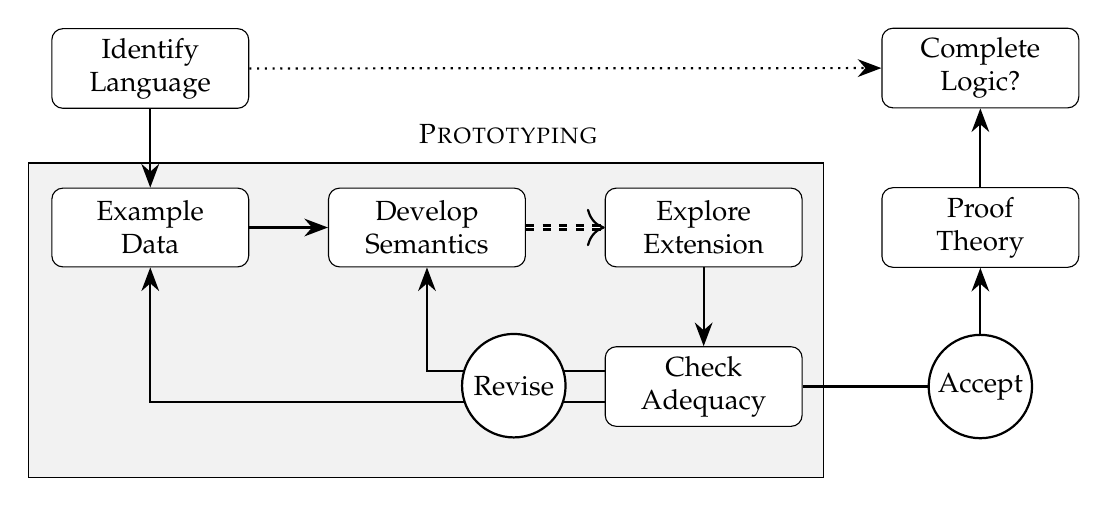
\begin{tikzpicture}[
		node distance=1cm,
		box/.style={
      draw,
      rounded corners,
      minimum width=2.5cm,
      minimum height=1cm,
      align=center,
      fill=white
    },
		arrow/.style={-{Stealth[length=3mm]}, thick}
		]

		\node[box] (lang) {Identify\\Language};

		\coordinate (core_pos) at ([xshift=-1.25cm,yshift=-1.5cm]lang);
		\coordinate (check_pos) at ([xshift=9.5cm,yshift=-3.4cm]core_pos);
		\node[above] at ([yshift=0.3cm]core_pos -| {$(core_pos)!0.5!(check_pos)$}) {\sc \strut\hspace{2cm} Prototyping};
		\draw[fill=gray!10] ([shift={(-0.3,0.3)}]core_pos) rectangle ([shift={(0.3,-0.3)}]check_pos);

		\node[box, below=of lang] (data) {Example\\Data};
		\node[box, right=of data] (model) {Develop\\Semantics};
		\node[box, right=of model] (ext) {Explore\\Extension};
		\node[box, below=of ext] (check) {Check\\Adequacy};
		\node[box, right=of ext] (proof) {Proof\\Theory};
		\node[box, above=of proof] (complete) {Complete\\Logic?};

		\draw[arrow] (lang) -- (data);
		\draw[arrow] (data) -- (model);
		\draw[arrow, double, dashed, ->] (model) -- (ext);
		\draw[arrow] (check) -| node[circle,draw,fill=white,pos=0.5,inner sep=2pt] {Accept} (proof);
		\draw[arrow] (proof) -- (complete);
		\draw[arrow] (ext) -- (check);
		\coordinate (check_up) at ([yshift=.2cm]check.west);
		\coordinate (check_down) at ([yshift=-.2cm]check.west);
		\draw[arrow] (check_up) -| (model);
		\draw[arrow] (check_down) -| node[circle,draw,fill=white,pos=0.1,inner sep=3pt,yshift=6pt] {Revise} (data);
		\draw[arrow, dotted] (lang) -- (complete);

	\end{tikzpicture}
\end{center}



\section*{Difficulties}%

\nicebox{
	The standard methodology has the following drawbacks:
	\begin{itemize}
		\item Computationally grueling to prototype semantic theories
		\item Problems of accuracy, redundancy, and memory
		\item Limits the development of complex semantic theories
		\item Restricts which language fragments can be studied/combined
	\end{itemize}
}


\section*{An Extended Methodology}%

\nicebox{
	Humans should not be carrying the computational load.
	\begin{itemize}
		\item SAT solvers, SMT solvers, Z3
		\item Examples: inequalities, bitvectors as states
		\item Z3 constraints as truth-conditions 
	\end{itemize}
}

\vspace{-.2in}

\begin{center}
	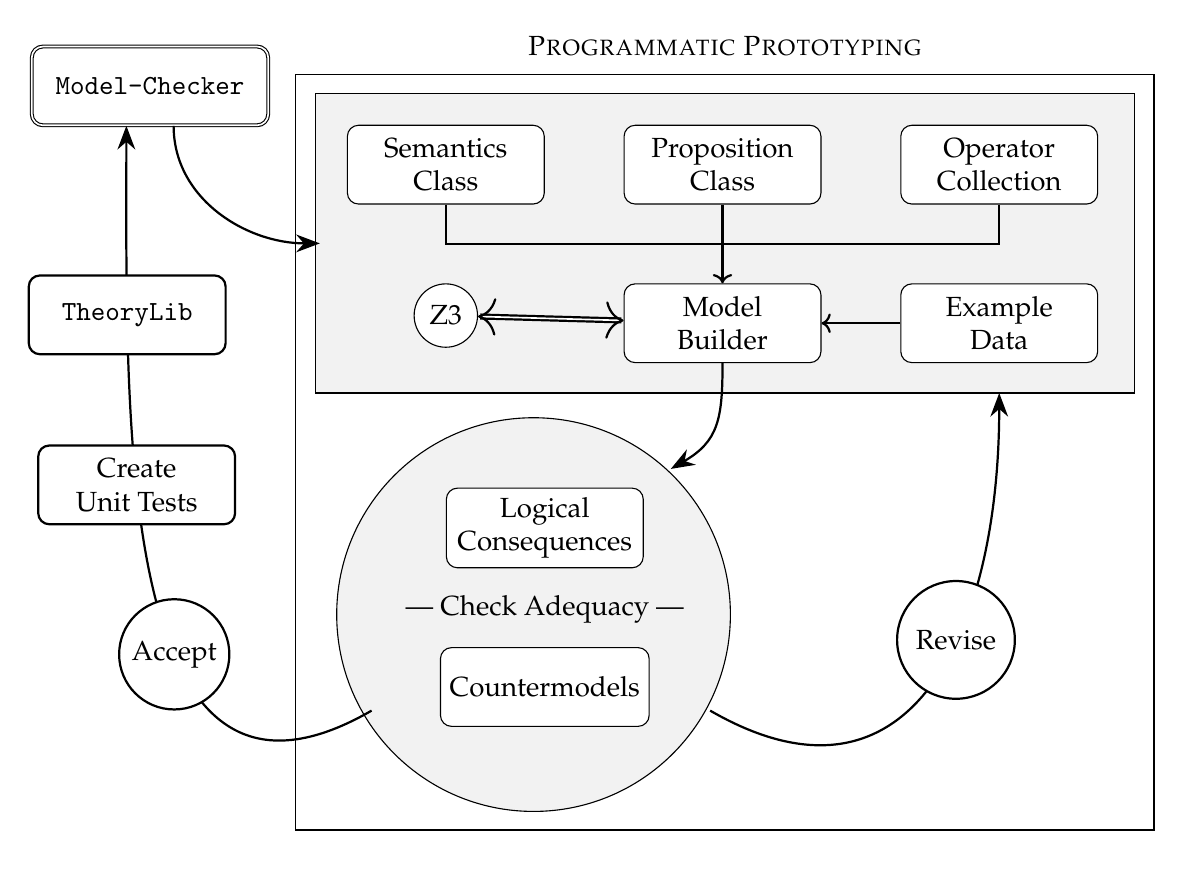
\begin{tikzpicture}[
		node distance=1cm,
		box/.style={
      draw,
      rounded corners,
      minimum width=2.5cm,
      minimum height=1cm,
      align=center,
      fill=white
    },
		arrow/.style={-{Stealth[length=3mm]}, thick}
		]

		\node[box, double] (model) {\tt ~Model-Checker~};

		\coordinate (below_model) at ([xshift=1.5cm,yshift=-1cm]model);
		\coordinate (core_pos) at ([xshift=2.4cm,yshift=-.4cm]model);
		\coordinate (check_pos) at ([xshift=9.8cm,yshift=-3.2cm]core_pos);
		\coordinate (big_top) at ([xshift=-.25cm,yshift=.25cm]core_pos);
		\coordinate (big_bot) at ([xshift=10.3cm,yshift=-9cm]big_top);
		\node[above] at ([yshift=0.4cm]big_top -| {$(core_pos)!0.5!(check_pos)$}) {\sc Programmatic Prototyping};
		\draw ([shift={(-0.3,0.3)}]big_top) rectangle ([shift={(0.3,-0.3)}]big_bot);
		\draw[fill=gray!10] ([shift={(-0.3,0.3)}]core_pos) rectangle ([shift={(0.3,-0.3)}]check_pos);

		\node[box, right=of below_model] (sem) {Semantics\\Class};
		\node[circle, draw, align=center, fill=white, below=of sem] (z3) {Z3};
		\node[box, right=of sem] (prop) {Proposition\\Class};
		\node[box, right=of prop] (ops) {Operator\\Collection};
		\node[box, below=of prop] (build) {Model\\Builder};
		\node[box, right=of build] (exp) {Example\\Data};

		\coordinate (below) at ([yshift=-2.6cm]build);
		\coordinate (top_left) at ([xshift=-4cm,yshift=.9cm]below);
		\coordinate (bot_right) at ([xshift=3.2cm,yshift=-4.0cm]top_left);
		\draw[fill=gray!10] ($(top_left)!0.5!(bot_right)$) ellipse (2.5cm and 2.5cm);
		% \node[below] at ($(top_left)!0.5!(bot_right) + (0,-2.8cm)$) {Check Adequacy};


		\node[box, left=of below] (thrm) {Logical\\Consequences};
		\node[below=0.22cm of thrm] (adeq) {--- Check Adequacy ---};
		\node[box, below=of thrm] (count) {Countermodels};
		\coordinate (revise) at ([yshift=-4.5cm]ops);
		% \node[box, below=of revise] (check) {Revise\\Semantics};

		\coordinate (box_in) at ([xshift=-1.6cm,yshift=-1cm]sem);
		\coordinate (model_out) at ([xshift=.3cm]model.south);
		\draw[arrow] (model_out) to[out=270,in=180] (box_in);

		\coordinate (cir_in) at ([xshift=1.6cm,yshift=.75cm]thrm);
		\draw[arrow] (build.south) to[out=-90,in=30,looseness=1.2] (cir_in);

		\draw[arrow, ->] (exp) -- (build);
		\coordinate (cir_out) at ([xshift=-2.2cm,yshift=-.3cm]count);
		\coordinate (model_in) at ([xshift=-.3cm]model.south);
		\draw[arrow] (cir_out) to[out=210,in=-90,looseness=1.2]
		node[box,draw,fill=white,pos=0.8,inner sep=3pt] {\tt TheoryLib}
		node[box,draw,fill=white,pos=0.62,inner sep=3pt] {Create\\Unit Tests}
		node[circle,draw,fill=white,pos=0.4,inner sep=3pt] {Accept}
		(model_in);

		\coordinate (cir_right) at ([xshift=4.3cm]cir_out);
		\coordinate (box_right) at ([yshift=-2.9cm]ops);
		\draw[arrow] (cir_right) to[out=-30,in=-90,looseness=1.4] node[circle,draw,fill=white,pos=0.6,inner sep=5pt] {Revise} (box_right);

		\draw[arrow, ->] (prop) -- (build);
		\draw[thick] (sem.south) |- ([yshift=.5cm]build.north);
		\draw[thick] (ops.south) |- ([yshift=.5cm]build.north);
		\draw[arrow, double, <->] (z3) -- (build);

	\end{tikzpicture}
\end{center}

\vspace{-20pt}

\section*{Conceptual Engineering}%

\nicebox{
	This methodology has the following advantages:
	\begin{itemize}
		\item Efficiently prototype new semantic theories
		\item Modular semantics, theory of propositions, operators
		\item Evaluate unified languages with many operators
		\item Compare rival theories over large data sets
	\end{itemize}
	Give it a try at: \href{https://pypi.org/project/model-checker/}{\texttt{https://pypi.org/project/model-checker/}}
}





\section*{Bilateral Propositions}%

Following \cite{Fine2017d,Fine2017,Fine2017a},  a \textit{modalized state space} is any $\mathcal{S}^\Diamond = \tuple{S,P,\sqsubseteq}$ where $\tuple{S,\sqsubseteq}$ is a complete lattice of \textit{states}, $P\subseteq S$ is a nonempty subset of \textit{possible states}, and $\sqsubseteq$ is the \textit{parthood relation} satisfying the following constraints:
  \begin{enumerate}[leftmargin=1.7in, itemsep=.05in]
    \item[\sc Nonempty:] $P \neq \varnothing$.
    \item[\sc Possibility:] If $s \in P$ and $t\sqsubseteq s$, then $t \in P$. 
  \end{enumerate}
The world states may then be defined, and a further constraint imposed:
  \begin{enumerate}[leftmargin=1.7in, itemsep=.05in]
    \item[\it Compatible:]  $s\circ t \coloneq s.t\in P$. 
    \item[\it World States:] $W \coloneq \set{w \in P\ |\ \forall s \circ w (s \sqsubseteq w)}$.
    \item[\sc World Space:] If $s \in P$, then $s \sqsubseteq w$ for some $w \in W$. 
  \end{enumerate}
A \textit{bilateral proposition} is any ordered tuple $\tuple{V,F} \in \mathbb{P}$ where
  \begin{enumerate}[leftmargin=1in, itemsep=.05in]
    \item[\it Closure:] $V, F \subseteq S$ are each closed under nonempty fusion.
    \item[\it Exclusive:] The states in $V$ are incompatible with the states in $F$.
    \item[\it Exhaustive:] Every possible state in $P$ is compatible with a state in $V$ or $F$.
  \end{enumerate}
A \textit{model} $\mathcal{M} = \tuple{S, P, \sqsubseteq, \vert{\cdot}}$ of $\mathcal{L}$ assigns each $\vert{p_i} = \tuple{\vert{p_i}^+, \vert{p_i}^-} \in \mathbb{P}$.
  \begin{itemize}[leftmargin=.25in, itemsep=.05in]
    \item $\vert{\neg A} = \tuple{\vert{A}^-, \vert{A}^+}$.
    \item $\vert{A\wedge B} = \tuple{\vert{A}^+ \otimes \vert{B}^+,  \vert{A}^- \oplus \vert{B}^-}$ where $X \otimes Y \coloneq \set{s.t \ |\ s \in X,\ t \in Y}$. 
    \item $\vert{A\vee B} = \tuple{\vert{A}^+ \oplus \vert{B}^+,  \vert{A}^- \otimes \vert{B}^-}$ where $X \oplus Y \coloneq X \cup Y \cup (X \otimes Y)$.
  \end{itemize}





\section*{Minimal Countermodels}%

\cite{Fine2012a} originally introduced a primitive \textit{imposition relation} $t \rightarrowtriangle_w u$ which indicates that ``$u$ is a possible outcome of imposing the change $t$ on the world [state] $w$'', and is subject to the following frame constraints on imposition:
  \begin{enumerate}[leftmargin=1.7in, itemsep=.05in]
    \item[\sc Inclusion:] If $t \rightarrowtriangle_w u$, then $t \sqsubseteq u$.
    \item[\sc Actuality:] If $t \sqsubseteq w$, then $t \rightarrowtriangle_w u$ for some $u \sqsubseteq w$. 
    \item[\sc Incorporation:] If $t \rightarrowtriangle_w u$ and $v \sqsubseteq u$, then $t.v \rightarrowtriangle_w u$. 
    \item[\sc Completeness:] If $t \rightarrowtriangle_w u$, then $u$ is a world-state. 
  \end{enumerate}
An abridged semantics for $\mathcal{L} = \tuple{\mathbb{L}, \neg, \wedge, \vee, \boxright}$ may then be stated as:
  \begin{itemize}[leftmargin=.5in, itemsep=.05in]
    \item $\mathcal{M}, w \vDash p_i$ \textit{iff} $s \in \vert{p_i}^+$ for some $s \sqsubseteq w$. 
    \item $\mathcal{M}, w \vDash A \boxright C$ \textit{iff} $\mathcal{M}, u \vDash C$ whenever $t \in \vert{A}^+$ and $t \rightarrowtriangle_w u$.
  \end{itemize}







\section*{Defining Imposition}%

\begin{enumerate}[leftmargin=1in]
  \item[\it Definition:] The frame constraints admit exceptions to $\Box A \coloneq \top \boxright A$.
  \item[\it State Space:] $P = \set{\square,\ a,\ b,\ c,\ b.c}$,\quad $W = \set{a,\ b.c}$, \quad $S/P = \set{a.b,\ a.c,\, a.b.c}$
  \item[\it Imposition:] $\rightarrowtriangle\ = \set{\
    \tuple{a,\ a,\ a},\ \tuple{b,\ b.c,\ b.c},\ \tuple{c,\ b.c,\ b.c},\\ 
    \strut\hspace{.46in} \tuple{\square,\ a,\ a},\ \tuple{\square,\ b.c,\ b.c},\ \tuple{\square,\ b.c,\ b.c}\ 
  }$
  \item[\it Interpretation:] $\vert{A} = \tuple{\set{a},\ \set{b.c}}$
  \item[\it Premise:] $\mathcal{M}, a \vDash \top \boxright A$ since the set of $\top$-alternatives to $a = \set{a}$.
  \item[\it Conclusion:] $\mathcal{M}, a \nvDash \Box A$ since $\mathcal{M}, b.c \nvDash A$.
\end{enumerate}
The definition $\Box A \coloneq \top \boxright A$ is preserved by the following definition of $\rightarrowtriangle$, where `$s \sqsubseteq_t w$' reads `$s$ is a $t$-\textit{compatible part} of $w$':
\begin{enumerate}[leftmargin=2in, itemsep=.05in]
  \item[\it Compatible Part:] $s \sqsubseteq_t w \coloneq s \sqsubseteq w \wedge s \circ t$. 
  \item[\it Maximal Compatible Parts:] $w_t \coloneq \set{s \sqsubseteq_t w \ |\ \forall r \sqsubseteq_t w (s \sqsubseteq r \rightarrow r = s)}$.
  \item[\it Imposition:] $t \rightarrowtriangle_w u \coloneq u \in W \wedge \exists s \in w_t(s.t \sqsubseteq u)$.
\end{enumerate}
We may then derive rather than posit the frame constraints on imposition, making the logic for $\boxright$ both stronger and more computable.

      

\section*{Computational Complexity as a Theoretical Virtue}%
\begin{enumerate}[leftmargin=1in]
	\item Z3 saves its `Function' objects as a mix of array-like and lambda-like objects.
	\item This means Z3 saves every value (that it is forced to for a given countermodel) for every input combination, meaning that the (worst-case) space complexity of functions is proportional to the input space. 
	\item Defining computational complexity: an algorithm takes $O(n)$ runtime or space if it scales linearly with some quantity $n$ as $n$ grows indefinitely large. 
	\item With inputs in $A \times B$, $A$ being the space of atomic sentences and $B$ the space of bitvectors, `verify' has a worst-case complexity of $O(\abs{A} \abs{B}) = O(\abs{A} 2^N)$, $N$ the size of the bitvectors.
	\item With inputs in $B^3$, `imposition' has a complexity of $O(2^{3N})$. 
	\item In practice, this means much slower runtimes for the imposition semantics: imposition semantics takes about 10 times as long as logos to run for $N=4$. 
	\item Since the complexity of `imposition' is exponential with $N$, this is only more marked for larger values of $N$, which can be useful for finding easily interpretable models. 
\end{enumerate}



\section*{Proofs}%

\begin{Pthm}[\sc Inclusion] \label{app:Inclusion}
  If $t \rightarrowtriangle_w u$, then $t \sqsubseteq u$.
\end{Pthm}

\begin{proof}
  Assuming $t \rightarrowtriangle_w u$, it follows that $u \in W$ where $s.t \sqsubseteq u$ for some $s \in w_t$.
  Since $t \sqsubseteq s.t$, it follows that $t \sqsubseteq u$ as desired. 
\end{proof}




\begin{Pthm}[\sc Actuality] \label{app:Actuality}
  If $t \sqsubseteq w$ and $w \in W$, then $t \rightarrowtriangle_w u$ for some $u \sqsubseteq w$. 
\end{Pthm}

\begin{proof}
  Assume $t \sqsubseteq w$ for $w \in W$. 
  Thus $w \in P$ where $w.t = w$, and so $w \circ t$.
  Since $w \sqsubseteq w$, we know $w \sqsubseteq_t w$.
  Let$r \sqsubseteq_t w$ where $w \sqsubseteq r$, and so $r \sqsubseteq w$, and so $w \in w_t$.
  Since $w.t \sqsubseteq w$, we know $t \rightarrowtriangle_w w$, and so $t \rightarrowtriangle_w u$ for some $u \sqsubseteq w$. 
\end{proof}





\begin{Pthm}[\sc Incorporation] \label{app:Incorporation}
  If $t \rightarrowtriangle_w u$ and $v \sqsubseteq u$, then $t.v \rightarrowtriangle_w u$. 
\end{Pthm}

\begin{proof}
  Assuming $t \rightarrowtriangle_w u$ and $v \sqsubseteq u$, we know $u \in W$ where $s.t \sqsubseteq u$ for some $s \in w_t$.
  Thus $s.t.v \sqsubseteq u$ and $s \sqsubseteq_t w$ where (1): $r \sqsubseteq s$ whenever $r \sqsubseteq_t w$ and $s \sqsubseteq r$.
  So $s \sqsubseteq w$.
  Since $u \in P$, we also know that $s \circ t.v$, and so $s \sqsubseteq_{t.v} w$.

  Let $q \sqsubseteq_{t.v} w$ where $s \sqsubseteq q$, and so $q \sqsubseteq w$ where $q \circ t.v$, and so $q.t.v \in P$. 
  Thus $q.t \in P$, and so $q \circ t$.
  It follows that $q \sqsubseteq_t w$, and so $q \sqsubseteq s$ follows from (1). 
  Generalizing on $q$, we know (2): $q \sqsubseteq s$ whenever $q \sqsubseteq_{t.v} w$ and $s \sqsubseteq q$.

  Having already shown that $s \sqsubseteq_{t.v} w$, it follows from (2) that $s \in w_{t.v}$.
  Since $s.t.v \sqsubseteq u$ for $u \in W$, we may conclude that $t.v \rightarrowtriangle_w u$ as desired. 
\end{proof}






% \begin{Pthm}[\sc Completeness] \label{app:Completeness}
%   If $t \rightarrowtriangle_w u$, then $u$ is a world-state. 
% \end{Pthm}
%
% \begin{proof}
%   Immediate from the definition of \textit{Imposition}.
% \end{proof}


\vfill

\bibliographystyle{Phil_Review} %%bib style found in bst folder, in bibtex folder, in texmf folder.
\nobibliography{Zotero} %%bib database found in bib folder, in bibtex folder


\end{document}
